\documentclass[12pt,twoside,slovak,a4paper]{article}

\usepackage[slovak]{babel}
\usepackage[T1]{fontenc}
\usepackage[utf8]{inputenc}
\usepackage{graphicx}
\usepackage{float}
\usepackage{url} % príkaz \url na formátovanie URL
\usepackage{hyperref} % odkazy v texte budú aktívne (pri niektorých triedach dokumentov spôsobuje posun textu)
\usepackage{setspace}
\usepackage{titlesec}
\usepackage{cite}
\usepackage{times}
\usepackage[dvips,dvipdfm,a4paper,centering,textwidth=15cm,top=3cm,headsep=.6cm,footnotesep=1cm,footskip=1cm,bottom=2cm]{geometry}


\graphicspath{ {images/} }


\begin{document}

\pagestyle{empty}

\begin{titlepage}
    \begin{center}
                 
        \LARGE{Slovenská technická univerzita} \\
        \LARGE{Fakulta informatiky a informačných technológii} \\      
        \Large{FIIT-XXX-YYY}
                
        \vspace{7cm}
        \Large{Richard Randák} \\ 
        \vspace{0.25cm}
        \huge{Spracovanie dopravnej siete}\\
        \vspace{0.25cm}
        \Large{Bakalárska práca} \vspace{0.25cm}
        
        
        \vfill    
            
    \end{center}
    \large
    Študijný program: Informatika\\
    Študijný odbor: 9.2.1 Informatika\\
    Miesto vypracovania: Ústav počítačových systémov a sietí, FIIT STU, Bratislava \\
    Vedúci práce: Ing. Dušan Bernát\\
    December 2015
    
\end{titlepage}

\begin{titlepage}
\setlength{\parindent}{0pt}
\Large
\textbf{Anotácia}
\normalsize
\newline
\newline
\begin{center}
Slovenská technická univerzita v Bratislave\\
FAKULTA INFORMATIKY A INFORMAČNÝCH TECHNOLÓGIÍ\\
Študijný program: Informatika\\
\end{center}

\textbf{Autor:} Richard Randák \\
\textbf{Bakalárska práca:} Spracovanie dopravnej siete \\
\textbf{Vedúci bakalárskej práce:} Ing. Dušan Bernát \\
\textbf{December 2015}
\newline
\newline
Cieľom bakalárskej práce je nájsť, získať a následne spracovať dáta reprezentujúce reálne dopravné siete. Pri analýze týchto sieti sa častokrát objavujú ich vlastnosti ako maximálny stupeň uzla, priemer siete alebo distribúcia stupňa vrcholov. Tie je možné získať práve transformáciou dopravnej siete do podoby grafu, teda množiny vrcholov a hrán.  Cieľom práce je teda tiež vytvorenie takého opisu grafu v textovom súbore, ktorý bude uľahčovať ďalšiu prácu alebo jeho podrobnejšiu analýzu. Praktická časť práce umožnuje modifikáciu výstupného formátu pre špecifickejšie použitie a získanie základných charakteristík spracovaných sietí.
\end{titlepage}

\begin{titlepage}
\setlength{\parindent}{0pt}
\Large
\textbf{Anotation}
\normalsize
\newline
\newline
\begin{center}
Slovak University of Technology Bratislava\\
FACULTY OF INFORMATICS AND INFORMATION TECHNOLOGIES\\
Degree Course: Informatics\\
\end{center}

\textbf{Author:} Richard Randák\\
\textbf{Bachelor Thesis:} Processing of transport network\\
\textbf{Supervisor:} Ing. Dušan Bernát\\
\textbf{ December 2015 }\\
\newline
\newline
First of the bachelor thesis goal is to find, to get and to process data representing real transport networks. There can be seen network properties like maximal node degree, graph diameter, or node degree distribution during analysis of these networks. We are able to get these properties from transformation of the network to a graph form, or to a set of nodes and edges. So, the goal of bachelor thesis is creating graph description, which will make further work or deeper analysis more easier. The practical part of the work will allow modification of the output format for more specific use, and to get basic characteristics of the processed network.
\end{titlepage}

\tableofcontents
\newpage
\setcounter{page}{1}
\setstretch{1.15}
\pagestyle{plain}
\newcommand{\sectionbreak}{\clearpage}

\section{Úvod}
V priebehu celej histórie ľudskej spoločnosti je vidieť snaha o spracovanie reálneho sveta do jednoduchšej podoby. Aby sa v ňom dalo lepšie orientovať, začali ľudia svoje okolie zakreslovať na kameň, či papier. Vznikali prvé mapy, teda jednoduchšia reprezentácia zložitej stavby sveta. Tie umožnovali lepšie plánovanie obchodnej či vojenskej stratégie. Stavba ciest vytvorila mapám ďalšie výhody a funkcie. Časom sa vybudovali cestné siete, v ktorých sa už dalo analyzovať ich vlastnosti, ktoré pomáhali riešiť zložité otázky. Napríklad otázka, kde postaviť vojenský tábor, z ktorého by sa dalo dostať do všetkých kritických oblastí čo najrýchlejšie. Alebo, ako naplánovať a synchronizovať trasy obchodných karaván tak, aby prešli všetky veľké mesta práve raz, a bez použitia nebezpečných ciest. Podobné problémy musíme riešit aj dnes.
	
	Dnešné dopravné siete sú veľmi komplikované a široké, preto je nutné ich analýzu automatizovať.  Jedným zo spôsobou je grafová reprezentácia siete, ktorá zachytáva vrcholy (uzly) a hrany (cesty) väčšinou aj s ohodnotením, napríklad dĺžkami ciest.  Pomocou výpočtových zariadení a algoritmou na prácu s grafmi vieme zistiť veľa zaujímavých vlastností. Z nich je možné  zefektívniť dopravu, rozhodnúť sa pre ideálnu lokáciu pre firemný sklad a podobne. 
	
	Aby mohol počítač s grafom pracovať, musí ho najskôr vedieť prečítať, napríklad z textového súboru. Formátou na uchovávanie grafu je však viacero, a rovnako tak je aj grafových typov.  Je preto potrebné rozhodnúť sa akú reprezentáciu si vybrať. Ešte predtým je nutné tieto dáta získať. Viaceré dopravné spoločnosti dátami o dopravných sietach disponujú, no nezverejnujú ich v čistej podobe. Väčšinou sú zverejnené cez webové stránky, na ktorých je možné vyhľadávať konkrétne stanice či zastávky (vrcholy) alebo aj spoje, teda cesty medzi nimi. To je našťastie všetko, čo nám k vytvoreniu grafu treba. 
	
	Kedže sú dnešné siete veľmi široké a husté, nie je možné prechádzať ručne stránkami a zapisovať si zobrazené informácie. Prechádzanie stránok musí byť automatické a naplánované tak, aby sa žiadne dáta nevynechali. Výsledkom komunikácie s takouto stránkov sú súbory, v ktorých je ešte treba požadované dáta lokalizovať.

\section{Zdroje}
Nutným vstupom pre spracovanie dopravnej siete sú dáta. Na ich získanie potrebujeme nájsť vhodný zdroj. Kedže na začiatku o dopravnej sieti nevieme vôbec nič, vhodný zdroj by mal umožnovať vyhľadávanie podľa číselného identifikátora alebo ideálne všetkých spojov bez obmedzení. Využiteľné sú aj zdroje, ktoré umožnujú vyhľadávanie spojov podľa názvu stanice. V takom prípade je však nutné k nim nájsť aj zoznam staníc v danej sieti, alebo zoznam vozidiel, podľa ktorých bude možné na stránke spoje vyhľadávať. Zdroj tiež nesmie využívať ochranu proti automatizovanému prístupu ako napríklad zadávanie kódu z obrázka.  Medzi vhodné zdroje teda patria najmä webové stránky železničných, autobusových či leteckých spoločností, ktoré slúžia zákazníkovi práve na vyhľadávanie a čítanie informácií o spojoch. Jednou z možností je tiež získanie dát z mapy, avšak tej sa pre jej zložitosť ďalej venovať nebudem.
	 \subsection{České dráhy}
	 Najvhodnejšími sa zdajú byť konkrétne stránky českého dopravcu \textbf{České Dráhy a.s.}, ktoré umožnujú vyhľadávanie spojov podľa identifikačnej masky prostredníctvom jednoduchého formulára ukázaného na obrázku.	
	 \begin{figure}[H]
	 \caption{Základný formulár}
	 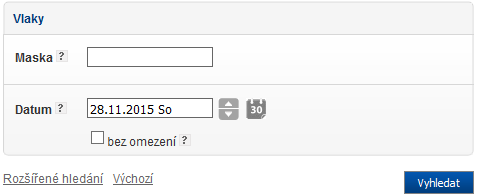
\includegraphics{cd_formular}
	 \end{figure}
	 Po vybraní voľby \emph{bez omezení}, sa zruší dátumové obmedzenie a následne po stlačení tlačidla \emph{Vyhledat} sa zobrazí zoznam všetkých spojov, ktoré vyhovujú zadanej maske. Formulár však umožnuje zadať aj prázdnu masku, čím by sa mal zobraziť kompletný zoznam všetkých spojov. Samozrejme zoznam je príliš dlhý a preto stránka umožnuje v zozname listovať cez odkazy \emph{předchozí} a \emph{následující}.  
	 \begin{figure}[H]
	 \caption{Zoznam spojov}
	 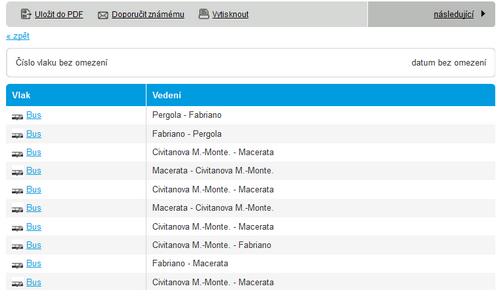
\includegraphics{cd_zoznam}
	 \end{figure}
	 Pri každom riadku v zozname je tiež odkaz na detailnejší opis príslušného spoja. V ňom vidíme všetky názvy staníc a zastávok, a taktiež príchody a odchody, z ktorých je možné vypočítať časovú dĺžku cesty medzi dvoma stanicami. Niektoré spoje majú aj údaje o dĺžky ciest medzi stanicami v kilometroch.  
	 \begin{figure}[H]
	 \caption{Detaily konkrétneho spoja}
	 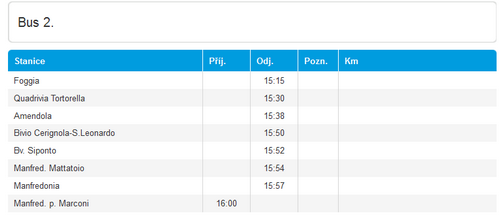
\includegraphics{cd_spoj}
	 \end{figure}
	 
	 Zdroj obsahuje všetky potrebné dáta k vytvoreniu grafu na reprezentáciu dopravnej siete.  Tento zdroj tiež disponujú dátami o rozsiahlej európskej dopravnej sieti, vrátane železničných, autobusových a dokonca aj lodných spojoch.
		 
	 \subsection{CP}
	 Ďalším vhodným zdrojom je stránka \textbf{cp.sk}, ktorá funguje na podobnom, ak nie rovnakom princípe ako stránky českých dráh. Prvotný formulár na vyhľadávanie spojou má rovnaký. Disponuje tiež podobnými dátami. Oproti stránkam českých dráh má naviac viacero samostatných cestovných poriadkov, vrátane MHD v slovenských mestách. Bohužial, pri zobrazení výsledkov nefunguje pokračovanie na ďalšie stránky v zozname, čo znemožnuje automatické spracovanie výsledkov.
	Stránka však umožnuje vyhľadávanie odchodov zo zadanej stanice, a odtiaľ ku konkrétnemu spoju. Na automatizované spracovanie je teda potrebné mať k dispozícii zoznam všetkých staníc v danej sieti. Formulár na takéto vyhľadavanie vyzerá následovne.
	\begin{figure}[H]
	 \caption{Formulár na vyhľadávanie podľa stanice}
	 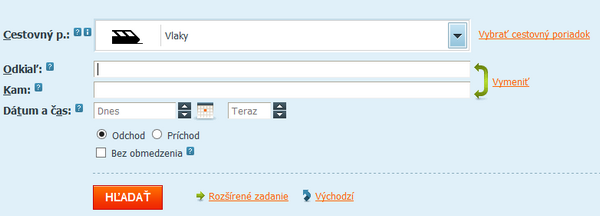
\includegraphics{cp_odchod_form}
	 \end{figure}
	 Vo formulári treba vyplniť buď políčko \emph{Odkiaľ}, alebo políčko \emph{Kam}. Následne sa zobrazí zoznam všetkých odchodov z danej stanice, resp. príchodov do danej stanice. V prípade voľby \emph{Bez obmedzenia} sa v zozname nachádzajú všetky možné odchody/príchody, teda aj tie, ktoré chodia len v určité dni.
	 	
	 \begin{figure}[H]
	 \caption{Odchody zo stanice Bacúch}
	 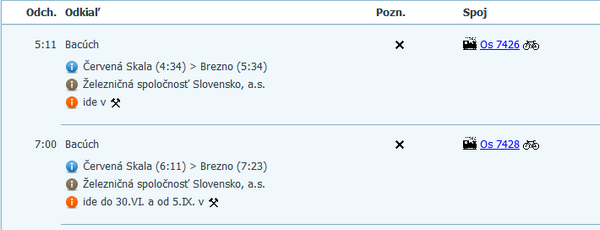
\includegraphics{cp_odchod_zoznam}
	 \end{figure}
	 
	 Po kliknutí na identifikačný názov spoja sa zobrazí celá trasa daného spoja, ktorú môžme konečne spracovať
	 
	 \begin{figure}[H]
	 \caption{Konkrétny spoj Os 7426}
	 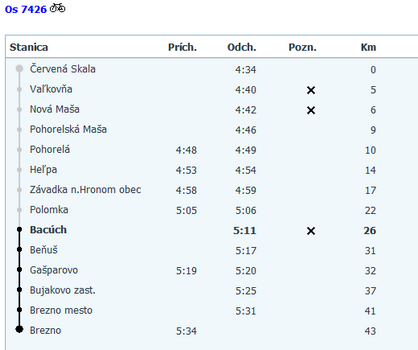
\includegraphics{cp_konk_spoj}
	 \end{figure}

	\subsection{Zelpage.cz}
	Webová stránka zelpage.cz sa zaoberá železničnou dopravou. Okrem článkov a fotografií je na stránke možné nájsť aj zoznam vlakových tratí pre viaceré európske štáty. Väčšina z týchto tratí má aj podrobný zoznam staníc a k nim aj vzdialenosť od začiatočnej stanice v kilometroch. Kedže ide o fyzickú trať a nie o konkrétny vlakový spoj, údaje o časovej vzdialenosti nie sú k dispozícii. Narozdiel od predošlých zdrojov, zelpage.cz umožnuje dostať sa k potrebným dátam cez GET žiadosť, teda jednoducho cez URL adresu.
	
		 
\section{Komunikácia s webom}
Komunikácia s webovým zdrojom prebieha cez protokol HTTP. Ten umožnuje dva typy metód žiadosti - \emph{GET request method} a \emph{POST request method}.  Zatiaľ čo pri GET metóde stačí len poslať URL reťazec s argumentami, pri POST metóde je to o čosi zložitejšie. Argumenty tejto metódy sú odosielané vrámci tela žiadosti. Je preto bezpečnejší a ťažšie sledovateľný. URL reťazce odosielané GET metódou je napríklad možné vidieť aj v histórii prehliadača a teda nie je vždy vhodná.

	\subsection{Webový formulár}
	Formulár je často používaným prvkom vo webových stránkach. Umožnuje používateľovi zadať údaje, podľa ktorých sa následne stránka zachová, alebo ktoré si ukladá. Najčastejšie reprezentuje vyhľadávací filter, alebo požaduje od používateľa prihlasovacie údaje, či kontakt.
	
	Webový formulár je definovaný značkou \texttt{<form>} a vo svojom tele obsahuje ďalšie webové komponenty, typicky kombináciu prvkov ako check-box, tlačidlo na potrvrdenie (submit button) a textové polia. Okrem komponentov má tiež vlastnosť \emph{action}, ktorá definuje \emph{form-handler}, teda typicky stránku so skriptom, ktorá rieši spracovanie vstupných údajou po odoslaní formulára. Odoslanie formulára sa aktivuje stlačením submit tlačidla. Nakoniec má ešte atribút \emph{method}, ktorý zas vyjadruje akou metódou sa budú dáta z formuláru odosielať. V podstate pri formuláry na odosielanie osobných údajou, pri ktorých nechceme, aby boli ľahko viditeľné ide o POST metódu, a pri filtroch, pri ktorých odosielané údaje nie sú zneužiteľné, sa väčšinou využíva GET metóda.
	
	Komponenty formulára sú definované značkou \texttt{<input>}, majú vlastnosť \emph{type}, ktorá určuje o aký komponent ide, napríklad \emph{text} na textové pole, alebo \emph{submit} na submit tlačidlo. Ďalšia dôležitá vlastnosť je \emph{value}, ktorá sa mení na základe interakcie používateľa s daným prvkom. Vlastnosť \emph{value} pri textovom poli teda vyjadruje reťazec zadaný používateľom do tohto poľa a zároveň reťazec, ktorý v ňom sa zobrazuje.
\newline \newline	
Príklad jednoduchého formuláru: 
\small
\begin{verbatim}
<form action= <"form_handler.php">   
  Message:<br> 
  <input type="text" name="message" value="Type a message here"> 
  <br><br> 
  <input type="submit" value="Submit">
</form> 
\end{verbatim}
\normalsize	

 \begin{figure}[H]
 	 \caption{Príklad formuláru}
 	 \centering
	 
\includegraphics{form_example}
 \end{figure}
	 
V tomto príklade po stlačení tlačidla sa spustí skript \emph{form\_handler.php}, ktorý rieši spracovanie napísanej správy. 


	\subsection{Webové tabuľky}
	Výstupom komunikácie so zdrojovou stránkou by mali byť HTML súbory obsahujúce potrebné dáta. Tie však treba v súbore ešte nájsť,identifikovať a osamostantiť. Dáta sa väčšinou vyskytujú ako prvky webovej tabuľky. Tabuľka je definovaná značkou \texttt{<table>}. Vo svojom tele využíva značky \texttt{<tr>} vyjadrujúce riadok v tabuľke. V nich už sú definované samotné dáta v úvodzovkách, ohraničené značkami \texttt{<td>} a \texttt{</td>} na vyjadrujenie prvku tabuľky.  

\section{Grafy v informatike}

\subsection{Teória grafov}
Graf je štruktúra, pozostávajúca z vrcholov (uzlov) a hrán spájajúcich tieto vrcholy \cite{ADM}. Formálne je to dvojica, tvorená množinou vrcholov a množinou hrán G = \{ V , E \}, kde množina hrán E je podmnožinou karteziánskeho súčinu množiny vrcholov. Z toho vyplýva, že hrana je definovaná dvojicou vrcholov, ktoré v grafe spája.
Ak ide o usporiadanú dvojicu, hrana je orientovaná, a usporiadanie určuje smer hrany. V neorientovanej hrane na usporiadaní nezáleží, a vyjadruje obojsmerné prepojenie vrcholov. Vrcholy alebo uzly predstavujú napríklad mestá, a hrany predstavujú cestné spojenia medzi nimi.  Podľa typu hrán, ktoré graf obsahuje, sa grafy delia tiež na viacero typov.

\begin{itemize}
\item \textbf{Obyčajný graf} obsahuje len neorientované (obojsmerné hrany). Hrana (A,B) teda vyjadruje spojenie z A do B a zároveň aj spojenie z B do A.
\item \textbf{Orientovaný graf} obsahuje len orientované (jednosmerné hrany). Hrana (A,B) teda vyjadruje len spojenie z A do B. Smer hrany je v grafickej reprezentácii grafu zobrazovaný šípkou. 
\item \textbf{Zmiešaný graf} obsahuje jednosmerné a aj obojsmerné hrany \cite{ADM}. 
\end{itemize}	

Je tiež možné, že medzi dvoma vrcholmi existuje viacero hrán. Ak to graf povoluje, nazýva sa \textbf{multigraf}.

Špeciálnou hranou je tzv. slučka, ktorá vyjadruje hranu spájajúca vrchol sám so sebou. Graf s takýmito hranami sa nazýva \textbf{pseudograf}. Aj keď je podľa definície grafu takáto hrana prijateľná, v reprezentácii reálneho sveta je väčšinou nepoužiteľná.

\subsubsection{Vlastnosti vrcholov}
Vrcholom v neorientovanom grafe je možné vypočítať napríklad stupeň vrchola, označujúci sa ako deg(v). Stupeň vrchola vyjadrujúce počet hrán, ktoré tento vrchol obsahujú \cite{KzDM}.  To znamená, koľko hrán daný vrchol spája s iným, resp. ak ide o slučku, so samým sebou.

Keďže v orientovanom grafe majú hrany aj smer, je možné túto vlastnosť rozdeliť na dve. 
\begin{itemize}
\item \textbf{vstupný stupeň vrcholu} vyjadruje počet hrán, ktoré do vrchola smerujú, teda v ňom končia
\item \textbf{výstupný stupeň vrcholu} vyjadruje počet hrán, ktoré z daného vrchola vychádzajú, teda smerujú do susedného vrchola
\end{itemize}

V cestnej sieti tieto vlastnosti môžu ovplyvniť zložitosť križovatky.

\subsubsection{Vlastnosti hrán}
Hrany v grafe môžu nosiť viacero vlastností. Hrany predstavujú napríklad železničné spojenia. Tie môžu byť samozrejme rôzne dlhé. Takáto vlastnosť hrany sa nazýva \textbf{váha} a hrana s váhou sa volá ohodnotená hrana. Podobne graf, ktorý má všetky hrany ohodnotené sa nazýva  \textbf{ohodnotený graf}.

V ohodnotenom grafe je už možné hľadať napríklad \textbf{najkratšiu cestu} medzi dvoma vrcholmi, čo je typickým problémom riešeným pomocou grafu.
\textbf{Cesta} v grafe je \textbf{sled} (postupnosť), v ktorom sú všetky hrany a zároveň aj všetky vrcholy rôzne \cite{ADM}. Dĺžka cesty je potom súčet cien hrán v tejto ceste.
\subsubsection{Meratelné vlastnosti grafu}
V zložitých grafoch je možné analyzovať a vypočítať rôzne vlastnosti grafu. 
\begin{itemize}
\item \textbf{Maximálny stupeň uzla} vyjadruje najvyššiu hodnotu stupňa vrchola v grafe
\item \textbf{Priemerný stupeň uzla} vyjadruje aritmetický priemer stupňa vrcholov v grafe
\item \textbf{Distribúcia stupňa vrcholov} je funkcia \emph{f(k)}, vyjadrujúca podiel vrcholov grafu so stupňom \emph{k}.
\item \textbf{Vzdialenosť vrcholov} je funkcia \emph{dg(u,v)} vyjadrujúca cenu najkratšej cesty spájajúcej vrcholy \emph{u} a \emph{v}.
\item \textbf{Priemer grafu} vyjadruje najväčšiu \emph{vzdialenosť vrcholov} v grafe.
\item \textbf{Priemerná dĺžka cesty} vyyjadruje priemernú \emph{vzdialenosť vrcholov} v grafe.

\item \textbf{Šírka bisekčného rezu (bisekcia)} 

\end{itemize}
Podobných vlastností je samozrejme omnoho viac, tieto sú však zaujímavé pre porovnávanie dopravných sieti.
	\subsection{Reprezentácia grafu}
	Samotný graf je abstraktná štruktúra. To znamená, že je nutné ju nejakým spôsobom reprezenzovať.
	\subsubsection{Grafická reprezentácia}
	Najčastejšou reprezentáciou grafu je pomocou obrázka. Čítať takto reprezentovaný graf dokáže aj človek, ktorý o grafoch veľa nevie. Uzly sú zobrazované ako zvýraznené body, častokrát s názvom alebo číslom. Hrany sú zobrazované ako čiary spájajúce tieto body. Smer hrany, pokiaľ ide o orientovanú hranu, je označený šípkou. Cena hrany je tiež zobrazená v blízkosti čiari, nesúvisí však s dĺžkou čiary.
	
	\begin{figure}[H]
 	 \caption{Neorientovaný neohodnotený graf}
 	 \centering
	 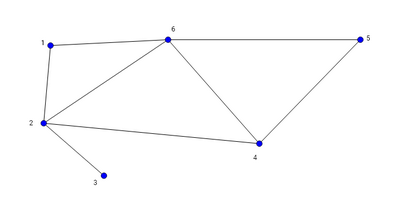
\includegraphics{neorientovany_small}
 \end{figure}
 
 \begin{figure}[H]
 	 \caption{Orientovaný ohodnotený graf}
 	 \centering
	 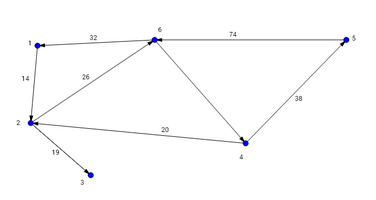
\includegraphics{orientovany_ohodnoteny_small}
 \end{figure}
  Graf môže byť tiež rovnako zobrazovaný aj v 3D priestore.
  
 	\subsubsection{Reprezentácia maticou}
 	Kedže grafová množina hrán je podmnožinou karteziánskeho súčinu vrcholov, je možné graf vyjadriť ako maticu týchto hrán, kde \emph{M[i][j]} bude vyjadrovať hranu \emph{(i , j)} teda hranu medzi vrcholmi \emph{i} a \emph{j}.
 	\textbf{Matica susednosti} vyjadruje či hrana \emph{(i , j)} existuje ( \emph{M[i][j] = 1} ) alebo nie ( \emph{M[i][j] = 0} ).
 	V prípade ohodnoteného grafu táto matica vyjadruje cenu hrany \emph{(i , j)}. Neexistujúca hrana sa označuje buď znakom pre nekonečno, alebo nulou. 
 	
 	Takáto reprezentácia nie je vždy efektívna, pretože zbytočne obsahuje záznam o všeetkých možných, a teda aj neexistujúcich hranách. V reálnych sieťach ktoré chceme grafom reprezentovať samozrejme nie sú spojené všetky vrcholy navzájom a takáto matica by bola pravdepodobne takmer celá zaplnená nulami resp. znakom pre nekonečno.
 	
	
	\subsubsection{Štandardné textové formáty}
	Ďalšou možnosťou reprezentácie je textový formát vyjadrujúci zoznam vrcholov a zoznam hrán grafu. Existuje už množstvo štandardných a používaných formátov. Formát tiež môže určovať alebo obmedzovať vlastnosti grafu, napríklad tým, že nepodporuje definovanie viacerých vlastností hrán.
	
\paragraph{Trivial Graph Format (TGF)} môže reprezentovaž orientovaný alebo neorientovaný graf. Je tvorený zoznamom vrcholov, teda dvojicami identifikačného čísla a názvu vrchola. Po vrcholoch následuje oddelovací znak '\#', a za ním zoznam hrán, teda dvojicou čisel vrcholov, ktoré hrana spája, a názvu tejto hrany.
\newline \newline 
Príklad: \newline	
\texttt{
1 Bratislava \newline
2 Košice \newline
3 Žilina \newline
\# \newline
1 3 cesta\_BA\_ZA \newline
2 1 cesta\_KE\_BA \newline
}
	
	\paragraph{Geographic Data File (GDF)} obsahuje zoznam vrcholov a ich vlastností,  ktoré sú definované na začiatku hlavičkou, podobne ako pri vytváraní tabuliek v databáze. Po vrcholoch je definovaná hlavička pre hrany, po ktorej následuje už zoznam hrán s ich vlastnostami. 
\newline \newline 
Príklad: \newline
\texttt{
nodedef>name VARCHAR,size DOUBLE, capital\_city BOOLEAN \newline
Bratislava,400.0,true \newline
Košice,250.0,false \newline
Praha,900.00,true \newline
edgedef>node1 VARCHAR,node2 VARCHAR, km\_length \newline
Bratislava,Košice,400 \newline
Košice,Praha,800 \newline
Bratislava,Praha,500 \newline
Praha,Bratislava,500 \newline
}


	\paragraph{Pajek NET} je jednoduchý formát, podobný formátu TGF. Obsahuje klúčový riadok \emph{*Vertices} , po ktorom následuje číslo vyjadrujúce počet vrcholov v grafe. Na ďalších riadkoch sú vyjadrené vrcholy, teda identifikačné číslo a názov. Po nich následuje kľúčové slovo \emph{*arcs} ak sú hrany v grafe orientované, a \emph{*Edges}  ak sú neorientované. Na ďalších riadkoch sú vyjadrené hrany, teda trojice čísel: číslo zdrojového vrchola, cieľového vrchola a hodnoty hrany, v našom príklade dĺžka v kilometroch. 
\newline \newline
Príklad: \newline
\texttt{
*Vertices 3 \newline
1 Bratislava \newline
2 Košice \newline
3 Žilina \newline
*arcs \newline
1 3 400 \newline
2 1 275 \newline
}

	\subsection{Nástroje na prácu s grafom} 
	S grafom definovaným v štandardnom formáte sa dá ďalej lahšie pracovať. Štandardné formáty sú tiež podporované rôznymi nástrojmi na prácu s grafmi. To môže byť často veľmi výhodné, najmä na náročné vypočty vlastností grafu, na ktoré treba poznať zložité a efektívne grafové algoritmy.
	
	\subsubsection{Pajek} 
	Pajek je program na analýzu a vizualizáciu rozsiahlych sietí s tisícami alebo až miliónmi vrcholov\cite{PAJEK}. Vznikol v novembri roku 1996. Implementovaný je v jazyku Delphi (Object Pascal). Je voľne dostupný pre nekomerčné účely. Program využíva na vstup Pajek NET formát, umožnuje však tiež zadať vstup cez maticu.
Hlavnými cieľmi programu sú: \cite{PAJEK}
\begin{itemize}
\item podporiť dekompozíciu veľkého grafu tak, aby bolo na prácu s nimi možné použiť vhodnejšie metódy
\item poskytnúť používateľovi silné nástroje na vizualizáciu
\item implementovať efektívne algoritmy na analýzu rozsiahlej siete
\end{itemize} 
	Dopravná sieť s ktorou budeme pracovať bude isto pozostávať z tisícky vrcholov medzi ktorými budú ešte husté cestné prepojenia. Nástroj Pajek bude preto určite jednou z možností, ako takúto sieť analyzovať, vypočítať potrebné vlastnosti a nakoniec aj zobraziť do grafickej podoby.
	
	\subsubsection{Gephi}
	Gephi je open-source softvér slúžiaci na analýzu a vizualizáciu sietí a grafov, podobne ako Pajek. Venuje sa ale podrobnejšie zobrazovaniu siete a manipulácii s jej komponentami. Využíva špeciálny engine na vykreslovanie siete v 3D prostredí v reálnom čase. Na vizualizáciu využíva grafickú kartu, preto je procesor počítača stále k dispozícii pre iné výpočty. Dokáže pracovať so sieťou o velkosti vyše 20 000 uzlov \cite{GEPHI}.   
	Projekt začal ako univerzitný projekt študentov vo Francúzku, implementovaný v jazyku Java. Neskôr bol vybraný do Google Summer of Code v rokoch 2009 až 2013.
	
	\subsubsection{GraphTool}
Graph-tool je nástroj vhodný na manipuláciu	a štatistickú analýzu grafou a sieti.
	
\section{Špecifikácia programu}

\subsection{Funkcionálne nároky}
\subsubsection{Výber zdroja}
Program musí byť schopný získavať dáta z viacerých webových stránok s umožniť používatelovi výber. To znamená, že zobrazí zoznam dostupných zdrojov, z ktorého si používatel jeden vyberie. Dáta z vybraného zdroja uloží do textového súboru. Pokiaľ už súbor s dátami vybraného zdroja existuje, dáta sťahovať nemusí. Používateľ však bude mať možnosť stiahnuť dáta nanovo, napríklad v prípade, že by sa dáta zo zdroja zmenili.
\subsubsection{Výber grafu}
Pre vybraný zdroj bude možné vybrať typ grafu. To znamená, že používateľ určí, či výsledný graf má obsahovať viaceré ohodnotenia hrán a taktiež či hrany majú byť orientované alebo neorientované. Okrem týchto možností, si používateľ bude môcť vybrať z dostupných grafových formátov, alebo vybrať vlastný formát. V prípade výberu vlastného formátu bude možné označiť vlastnosti hrán, ktoré chce používateľ do výstupého súboru uložiť - priemernú, minimálnu, maximálnu váhu, a taktiež aj možnosť uložiť všetky ohodnotenia. Po nastavení vlastností, program dáta vybratého zdroja spracuje do formy grafu. Po vytvorení grafu ho zapíše do textového súboru vo formáte vybraného používateľom. 
\subsubsection{Zhrnutie vlastností}
Pre vytvorený grafový súbor program spustí analýzu daného grafu. Na to môže využiť externé programy. Z výsledkov analýzy vytvorý zhrnutie a to spracuje do bežne používaného formátu, napríklad HTML. Toto zhrnutie vlasností siete, ktorú graf reprezentuje, musí obsahovať minimálny, maximálny a priemerny stupeň vrchola ako aj distribúciu stupňa vrcholov v podobe histogramu.
\subsection{Jazykové nároky}
Program bude komunikovať s webovými stránkami a teda vhodný jazyk musí umožnovať komunikáciu cez HTTP protokol. Taktiež musí poskytovať vhodné dátové štruktúry na dočasné uloženie a uchovávanie dát s ktorými pracuje. Užitočným bonusom sú aj jednoduché a bezpečné metódy na čítanie a zapisovanie do súboru. Taktiež je potrebné aby jazyk poskytoval funkcie na prácu s textom, keďže bude potrebné dáta hľadať v HTML súboroch

Pri sťahovaní dát zo stránok je potrebné nejaký čas medzi požiadavkami čakať, aby program simuloval bežného užívateľa. Preto je rýchlosť ďalšieho spracovania dát zanedbateľný. Jazyk teda môže byť pomalší.
\subsubsection{Java}
Jedným z vhodných jazykov je objektovo-orientovaný jazyk Java. Je široko využiteľný a disponuje balíkmi na komunikáciu s webom a odosielanie HTTP žiadostí, konkrétne java.net balík. Podporuje regulárne výrazy pri práci s textom. Ponúka balík s dátovými štruktúrami, konkrétne napríklad zoznamy a tabuľky v java.util balíku. Kedže ide o jazyk zameraný na objekty, umožnuje vytvorenie vlastného objektu na reprezentáciu vrcholu či hrany a teda aj celého grafu. Výhodou tohto jazyka je aj pohodlná práca so súbormi, konkrétne v rámci java.io balíka. Ďalšiou výhodou je možnosť jednoduchej implementácie viacerých vlákien. 
	Java je interpretovaný jazyk. Nevýhodou je teda jeho nižšia rýchlosť, ktorá však v našom prípade nie je nutná.

\section{Štruktúra programu}

Program bude pozostávať z troch samostatných hlavných častí. Každá časť vytvorí výstup, ktorý bude vstupom do následujúcej časti. 

	\begin{figure}[H]
	 \caption{Návrh štruktúry programu}
	 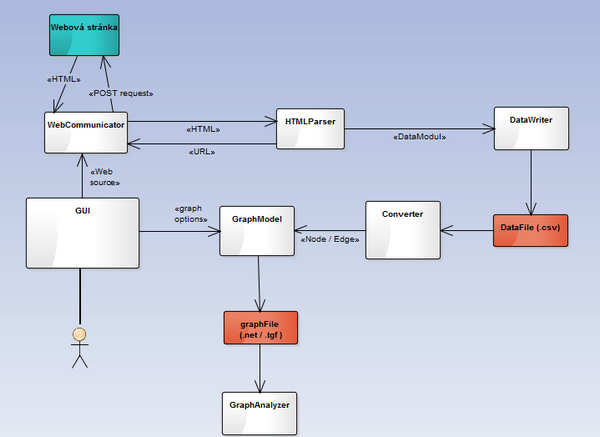
\includegraphics{prog_struct2}
	 \end{figure}
			
	\subsection{DataCollector}
	Prvá časť bude mať na starosť komunikáciu s webovou stránkou, zozbieranie potrebných dát a ich zápis do textového súboru v jednoduchšom a prehľadnejšom formáte, napríklad CSV. Najprv vytvorí spojenie so stránkou, odosiela žiadosti, ktorýmí sa dostane k HTML súborom s dátami. V nich podľa kľúčových slov či znakov nájde výskyt potrebných dát. Identifikuje ich, a zapíše do svojho súboru. Takto pokračuje kým zozbiera a zapíše všetky dáta o dopravnej sieti zo stránky.
	 
		\subsubsection{WebCommunicator}
		WebCommunicator bude modul v prvej časti programu. Jeho úlohou bude vytvárať HTTP requesty a získavať požadované HTML súbory. Využívať bude balíky potrebné na webovú komunikáciu. Úlohou tejto časti programu je teda napríklad potvrdzovanie formuláru na stránke. Kedže každý zdroj má iný prístup k údajom, každý zdroj bude mať túto časť inú.
				
		\subsubsection{HTMLParser}
		Ďaľším modulom je HTMLParser. Jeho úlohou bude prechádzať HTML súbory a hľadať potrebné údaje. Napríklad odkaz na ďalšiu stranu v zozname, alebo odkaz na detaili spoja. Taktiež bude musieť vedieť identifikovať a osamostatniť dáta z webovej tabuľky. Využívať bude teda balík na prácu so súbormi a textom.

Každý zdroj má uložené dáta v tabuľkách inak, a teda je nutné mať taktiež pre každý zdroj iný parser. Štruktúra stránky je však väčšinou podobná, čiže každý parser bude obsahovať funkciu na hľadanie odkazov v tabuľke spojov, a potom funkciu na parsovanie údajov v tabuľke konkétneho spoja.

		\subsubsection{DataWriter}
		Posledným modulom prvej časti je DataWriter, ktorý získanú skupinu dát upraví do praktickejšej, napríklad odstráni nechcené znaky v názvoch. Následne tieto dáta umožní zapísať do súboru v požadovanom zovšeobecnenom formáte, v našom prípade skupinu dát zapíše na samostatný riadok s dátami oddelenými bodkočiarkami. Forma výstupného súboru bude vyzerať takto:
	\small
		\begin{verbatim}
ROUTE;typ_spoja_1;
stanica_1;čas_odchodu_1;čas_príchodu_1;dĺžka_v_KM_1;
stanica_2;čas_odchodu_2;čas_príchodu_2;dĺžka_v_KM_2;
stanica_3;čas_odchodu_3;čas_príchodu_3;dĺžka_v_KM_3;
stanica_4;čas_odchodu_4;čas_príchodu_4;dĺžka_v_KM_4;
END_ROUTE;
ROUTE;typ_spoja_2;
stanica_5;čas_odchodu_5;čas_príchodu_5;dĺžka_v_KM_5;
stanica_6;čas_odchodu_6;čas_príchodu_6;dĺžka_v_KM_6;
stanica_7;čas_odchodu_7;čas_príchodu_7;dĺžka_v_KM_7;
stanica_8;čas_odchodu_8;čas_príchodu_8;dĺžka_v_KM_8;
END_ROUTE;
		\end{verbatim}
	\normalsize	
	
Konkrétny súbor s dátami zo stránky českých dráh vyzerá takto:	
		\small
		\begin{verbatim}
ROUTE;Bus;
Pergola;;6:54;0;
Bellisio Solfare;6:58;6:59;0;
Monterosso Marche;7:07;7:08;0;
Sassoferrato-Arcevia;7:14;7:15;0;
Melano-Marischio;7:23;7:24;0;
Fabriano Ca'Maiano;7:25;7:26;0;
Fabriano;7:38;;0;
ROUTE;Bus;
Fabriano;;13:45;0;
Sassoferrato-Arcevia;14:01;14:02;0;
Monterosso Marche;14:12;14:13;0;
Bellisio Solfare;14:21;14:22;0;
Pergola;14:28;;0;
		\end{verbatim}
	\normalsize	
Slovo 'ROUTE' v texte vyjadruje začiatok nového spoja, za ním následuje typ spoja, a na ďalších riadkoch sú údaje o zastávkach získané priamo zo stránky - názov, čas príchodu, čas odchodu a kilometrová vzdialenosť od prvej stanica. Koniec spoja vyjadruje kľúčové slovo END\_ROUTE.
	
	Pre potreby zdroja zelpage.cz bolo potrebné formát rozšíriť o možnosť vnoreného spoja, začínajúci slovom SUB\_ROUTE a končiaci slovom END\_ROUTE.
	
	\small
		\begin{verbatim}
ROUTE;vlak_110;
Bratislava hlavná stanica;;;0;
Bratislava-Železná studienka;;;3;
...
Devínske Jazero;;;17;
SUB_ROUTE;vlak_110;
Devínske Jazero;;;0;
Stupava;;;2;
END_ROUTE;
Zohor;;;26;
Plavecký Štvrtok;;;31;
...
Kúty;;;64;
Brodské;;;68;
Kúty štátna hranica;;;71;
END_ROUTE;

\end{verbatim}
	\normalsize	
	
	\subsubsection{InputGUI}
	Na výber zdroja poslúži grafické rozhranie modulu InputGUI. Umožní vybrať jeden z dostupných webových zdrojov, a tiež rozhodnúť, či má program dáta sťahovať nanovo, alebo použiť už uložený súbor s dátami. 
	
	\begin{figure}[H]
	 \caption{Návrh formuláru na vybratie zdroja dát}
	 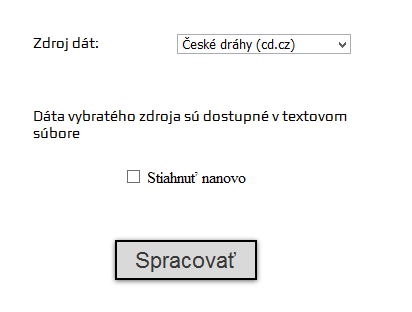
\includegraphics{gui_vyber_zdroja}
	 \end{figure}	
		
	\subsection{GraphBuilder}
	Druhá časť bude pracovať už len s lokálnym súborom vytvoreným v prvej časti. Postupne bude načítavať dáta a vytvárať z nich graf s viacerými ohodnoteniami hrán. Podľa nastavení od používatela nakoniec vygeneruje tento graf v takom formáte, aký je potrebný. Výsledný graf teda môže byť orientovaný alebo neorientovaný. Taktiež vo výstupe budú použité vybrané ohodnotenia hrán. Či už to bude dĺžka cesty, čas trvania cesty, priemer, suma, minimum, maximum týchto hodnôt, alebo aj všetky za sebou. Samozrejme, ak to daný grafový formát dovoľuje.
	
		\subsubsection{DataReader}
		DataReader je modul, ktorý dokáže vytvorený súbor z prvej časti čítať a logicky posielať dáta ďalej na spracovanie.  
		\subsubsection{Converter}
		Úlohou tohto modulu je získané dáta o staniciach či cestách pospájať. Údaje, ktoré dostane, obaluje do objektou reprezentujúcich vrchol či hranu v grafe. Po obalení a prepojení ich kontroluje, a detekuje tak možné chyby, respektíve nevyhovujúce vlastnosti ako záporná váha hrany. Po okontrolovaní a v prípade, že sú údaje v poriadku, ich odovzdáva ďalšiemu modulu.
		
		Presnejšie to znamená, že z každého záznamu o stanici vytvorí uzol s názvom stanice a odošle ho do modulu s databázou. Medzi každými dvoma za sebou idúcimi stanicami vytvorí hranu. Z času odchodu zo stanice A a času príchodu do následujúcej stanice B vypočíta časovú náročnosť hrany (A,B). Podobne vypočíta aj dĺžku tejto hrany v kilometroch. Obe hodnoty pridá k vytvorenej hrane. Výsledné hrany tiež odošle do modulu s databázou.

	
		\subsubsection{GraphModel}
		Dôležitým modulom v druhej časti je GraphModel, čiže modul, ktorý reprezentuje graf. Jeho súčasťou sú dátové štruktúry na uchovávanie vrcholov a hrán. Taktiež obsahuje nastavenia grafu, podľa ktorých rozhoduje, či nový vrchol alebo hranu do grafu pridať, alebo v prípade, že už daný vrchol či hranu graf obsahuje, rozhodnúť, ako ovplyvnia graf. Napríklad ak má byť graf orientovaný a obsahuje už hranu A => B, novú hranu B => A už pridávať nemusí. Čo však využiť môže, sú ohodnotenia tejto novej hrany, ak graf povoluje používať viaceré ohodnotenia pre hranu. Tento modul tiež musí obsahovať metódy na zapísanie grafu do rôznych formátov. 
		\subsubsection{InputGUI}
		Na vloženie požiadaviek výsledného grafu bude slúžiť modul InputGUI. Bude predstavovať základé grafické používateľské rozhranie. Umožní používateľovi vybrať požadovaný štandardný formát grafu alebo tiež vybrať požadované vlastnosti hrán, ktoré chce používateľ vo výstupnom neštandardnom grafe mať obsiahnuté.
	
	 \begin{figure}[H]
	 \caption{Návrh formuláru na vytvorenie grafu}
	 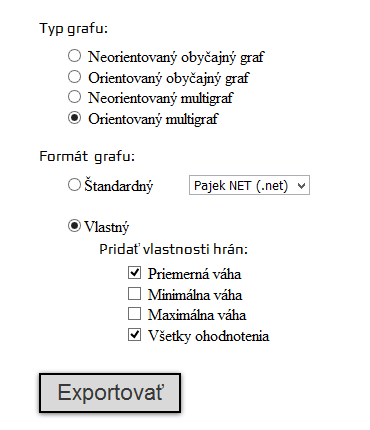
\includegraphics{gui}
	 \end{figure}
	 
	\subsection{GraphAnalyzer}
	Tretia časť bude pracovať so súbormi vytvorenými druhou časťou. Bude umožnovať výpočet požadovaných informácii, vlastností a tiež štatistiky z grafu. Na výpočet môže použiť externé programy špecializované a optimalizované na tieto výpočty.
	
	\section{Implementácia}
	Prvá a druhá časť programu bude implementovaná v jazyku Java v prostredí Eclipse. Využívať budeme balík na prácu s textom \emph{java.io} a balík \emph{java.net} na komunikáciu s webom. Táto kapitola ďalej popíše detailné riešenie problémov s ukážkami zo zdrojového kódu.
	 
%\acknowledgement{Ak niekomu chcete poďakovať\ldots}

% týmto sa generuje zoznam literatúry z obsahu súboru literatura.bib podľa toho, na čo sa v článku odkazujete
\nocite{*}
\bibliography{literatura}
\bibliographystyle{plain} % prípadne alpha, abbrv alebo hociktorý iný
\end{document}

